\chapter{Estado del arte}
\label{cap:capitulo2}
\setcounter{page}{1}

\begin{flushright}
\begin{minipage}[]{10cm}
\emph{Eres el amo de tu destino, el capitán de tu alma.}\\
\end{minipage}\\

Napoleon Hill, \textit{Piense y hágase rico}\\
\end{flushright}

\vspace{1cm}



En este capítulo se definirán algunos de los trabajos que han tenido más importancia en este proyecto. A lo largo de esta sección, se han revisado áreas con el propósito de comprender y aplicar conceptos clave en la creación del sistema como el control de motores a través de señales PWM, una interfaz HRI amena para poder comunicarse con el robot, modelos de aprendizaje automático para el reconocimiento de órdenes mediante comandos de voz, posicionamiento en interiores a partir de señales de \hyperlink{RSSI}{RSSI} y algoritmos de planificación de rutas para navegar en interiores. Todo esto, a su vez deberá ir integrado en una CPU de baja capacidad como la de la Raspberry Pi, ya que es un prototipo de bajo coste.\\

A pesar de ello, el sistema se diseñará para maximizar la eficiencia con los recursos disponibles, garantizando un equilibrio entre coste y funcionalidad. Esto llevará a soluciones innovadoras en el diseño del hardware y la optimización del software, permitiendo que el robot sea viable sin necesidad de componentes de alto coste.\\

En \cite{9815716}, se presentan diferentes alternativas sobre cómo controlar motores de corriente continua mediante señales PWM a los microcircuitos o, en este caso, motores reductores mediante un módulo controlador de motor L298N puede regular la velocidad y la dirección en ambos sentidos de los motores al mismo tiempo, lo cual es muy importante, ya que de esta manera no haría falta sincronizar ambos motores de ninguna manera.\\

Por otra parte, se necesitará averiguar qué modelo de aprendizaje automático (Figura \ref{fig:random_forest}) es el ideal para poder clasificar correctamente comandos por voz en diferentes clases, lo cual es fundamental para desarrollar una interfaz HRI amena que permita una comunicación efectiva con el robot. Esto se presenta en \cite{Zenkov-sklearn-SER-basics}, donde se ofrecen diferentes técnicas que se pueden aplicar a problemas de clasificación, regresión y técnicas de ingeniería de características para datos de audio. Además, se ofrece un vistazo en profundidad a la lógica, los conceptos y las propiedades de las redes neuronales profundas actuales, proporcionando información clave sobre algunos modelos de aprendizaje automático y la lógica en la elección de sus hiperparámetros, cuyo objetivo es reconocer comandos de audio por voz, permitiendo al robot comprender y ejecutar órdenes dadas por el usuario.\\

\begin{figure} [H]
  \begin{center}
    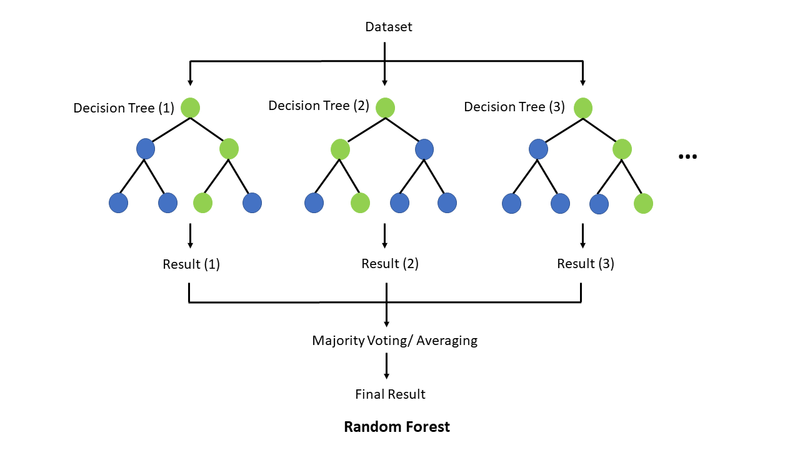
\includegraphics[scale=0.8]{figs/random_forest}
  \end{center}
  \caption{Algoritmo de aprendizaje automático Random forest.}
  \label{fig:random_forest}
\end{figure}\

De manera similar, el aprendizaje automático también desempeña un papel fundamental en la localización interna del robot, donde se emplean técnicas avanzadas para estimar su posición precisa en entornos interiores. Para poder determinar la posición precisa del robot, es necesario hacer uso de técnicas de localización interna. En este otro artículo \cite{unknown} se realiza un estudio sobre los sistemas de posicionamiento en interiores de "fingerprinting"(Figura \ref{fig:wifi}) que utiliza modelos de aprendizaje automático para crear un mapa de ubicación RSSI del entorno para una mejor estimación de la ubicación y que a diferencia de los sistemas de posicionamiento en interiores \hyperlink{BLE}{BLE} que se han implementado con modelos de pérdida de propagación, los cuales han demostrado estimar posiciones con grandes errores debido a la incertidumbre de las señales RSSI causadas por obstáculos interiores y fenómenos electromagnéticos, los de fingerprinting consiguen una mejor estimación de la posición. Para demostrarlo, se probarán diferentes hipótesis, como las siguientes:

\begin{enumerate}
 \item ¿La precisión de las balizas BLE escala linealmente con la cantidad de las mismas?
 \item ¿La precisión aumenta
cuando la distancia mínima entre dos posiciones es de 1 m mientras que el área de mapeo no cambia?
\end{enumerate}\ 

\begin{figure} [H]
  \begin{center}
    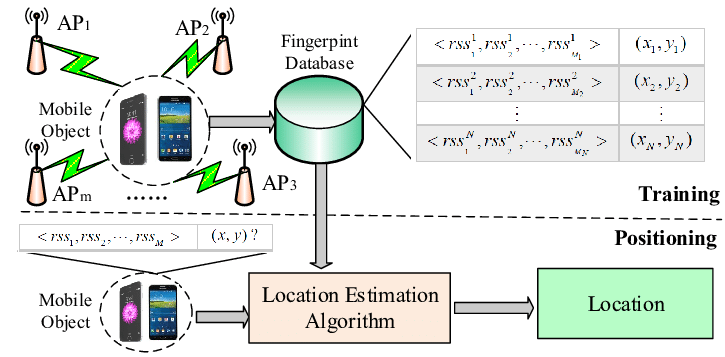
\includegraphics[scale=0.6]{figs/wifi}
  \end{center}
  \caption{Principio de WiFi fingerprinting.}
  \label{fig:wifi}
\end{figure}\

Los resultados de ambas hipótesis fueron verdaderas, por lo que para este proyecto servirá de gran ayuda para saber con precisión cuántos puntos de acceso WiFi son necesarios para un entorno. En este caso no se usarán balizas Bluetooth pero el procedimiento sería el mismo. Para poder estimar la posición del robot en el mapa mediante balizas WiFi, se hará uso de la trilateración (Figura \ref{fig:trilateration}), la cual es una técnica presentada y estudiada en este artículo \cite{inproceedings}. En él, se presenta un método basado en WiFi para el posicionamiento en interiores utilizando mediciones de intensidad de señal recibida (RSSI). También se estiman las distancias entre los puntos de acceso (\hyperlink{APs}{APs}) y el dispositivo móvil a partir de valores RSS evaluados por el modelo de propagación de la señal. Esto servirá para calcular, mediante diferentes fórmulas, la posición del robot en el mapa conociendo a su vez la posición de las balizas y ver cuánto error hay en la estimación.\\


\begin{figure} [H]
  \begin{center}
    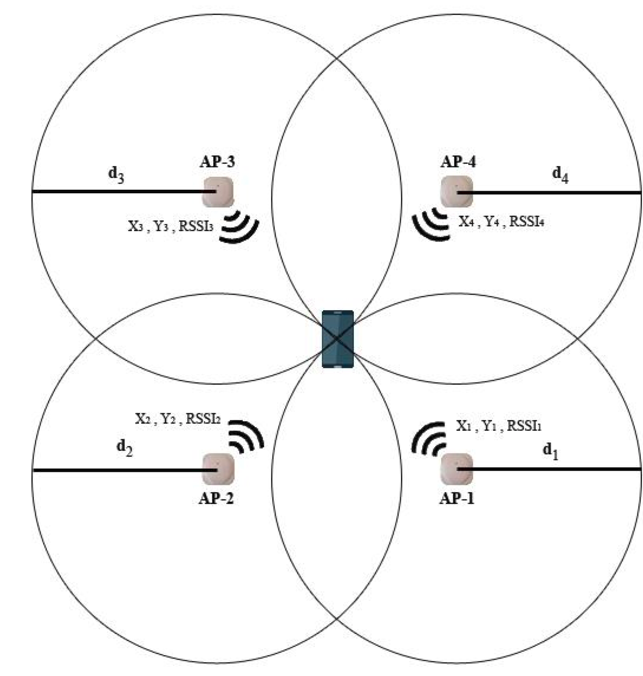
\includegraphics[scale=0.4]{figs/trilateration}
  \end{center}
  \caption{Técnica de trilateración por WiFi.}
  \label{fig:trilateration}
\end{figure}\

Una vez conocida la posición del robot, es importante que pueda planificar la ruta de manera eficiente en el entorno. Para ello, los algoritmos de planificación de rutas juegan un papel esencial. Este artículo \cite{article} sirve como introducción al concepto de planificación de rutas y navegación en el contexto de la robótica, presentando algoritmos y casos de uso donde los especialistas en robótica pueden desarrollar aplicaciones de búsqueda o planificación de rutas. En ese artículo, también se describen las características del algoritmo de búsqueda A* (Figura \ref{fig:astar}) y sus aplicaciones para un sistema de navegación para vehículos robóticos, y es el que se usará en este trabajo por su optimización, precisión y eficiencia en tiempo de ejecución.

\begin{figure} [H]
  \begin{center}
    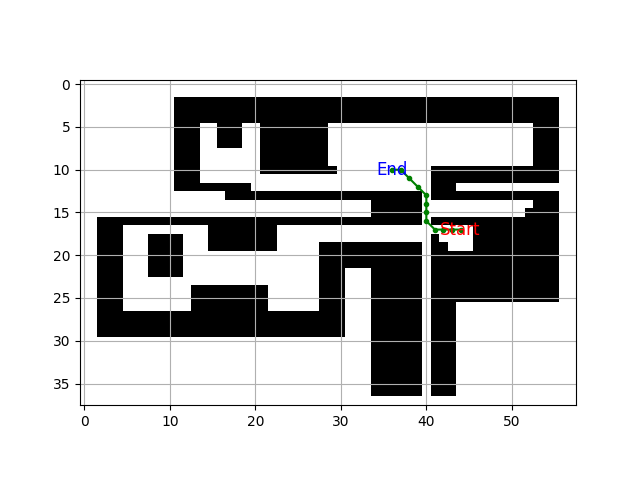
\includegraphics[scale=0.4]{figs/astar}
  \end{center}
  \caption{Algoritmo de búsqueda A*.}
  \label{fig:astar}
\end{figure}\

Una vez se ha entendido el concepto de planificación de rutas, el robot debe saber cómo desplazarse por la misma, siendo capaz ya de desplazarse en línea recta y de localizarse, pero se tienen en cuenta los giros que debe hacer en la ruta, por lo que se hará uso de un magnetómetro para conocer el ángulo de orientación del robot y así hacer giros más precisos. Otro paso importante, como se puede apreciar en este documento \cite{Ozyagcilar2015}, son las diferentes técnicas para la calibración del sensor, en el cual se proporciona la teoría para la calibración de una brújula electrónica de un teléfono inteligente para mitigar los efectos de hard y soft-iron, los cuales son los efectos producidos por materiales ferromagnéticos y que pueden magnetizarse sobre el magnetómetro.\\

Para poder garantizar que las lecturas del magnetómetro sean correctas y precisas y no se vean afectadas por ruidos o fluctuaciones, también sería necesario entender el uso de un filtro de paso bajo, como se explica en este otro artículo \cite{low_pass_filter}. Este filtro es fácil de implementar ya que utiliza pocos recursos y, con dos parámetros fáciles de comprender, resulta fácil de ajustar. A diferencia de otros filtros, este tiene menos desfase, lo cual lo convierte en una buena opción para suavizar las lecturas del magnetómetro y permitir que el robot realice giros mucho más precisos.



\vspace{15cm} % Espacio vertical de 1 cm







